    \textbf{Задание №3.} С помощью отладчика определить местонахождение переменных, строк и массивов в сегменте данных, а также их размер. Составить таблицу и подробное описание ячеек  сегмента данных (как в примере).\label{sec:3}

        \begin{table}[h!]
        \centering
        \renewcommand{\arraystretch}{1.3}
        \caption{Переменные сегмента данных}
        \label{tab:variables}
        \begin{tabular}{|c|c|c|c|p{6cm}|}
        \hline
        Переменная & Нач. адрес & Кон. адрес & Байт & Описание \\
        \hline
        \cellcolor{yellow} \texttt{\_} & 00403000 & 00403001 & 2 & символы возврата каретки (13), перевода строки (10) \\
        \hline
        \cellcolor{pink} \texttt{printf} & 00403002 & 0040300B & 11 & форматная строка для функции printf \\
        \hline
        \cellcolor{purple!30} \texttt{\_} & 0040300C & 0040300C & 1 & Окончание строки (0) \\
        \hline
        \cellcolor{blue!30} \texttt{a} & 0040300D & 0040300E & 2 & 2-байтовая переменная со значением 5 \\
        \hline
        \cellcolor{red} \texttt{b} & 0040300F & 00403012 & 4 & 4-байтовая переменная со значением 60 \\
        \hline
        \cellcolor{green} \texttt{r} & 00403013 & 00403016 & 4 & неинициализированная 4-байтовая переменная \\
        \hline
        \cellcolor{cyan} \texttt{dqq} & 00403017 & 0040301E & 8 & 8-байтовая вещественная переменная со значением 171.233 \\
        \hline
        \multicolumn{3}{|c|}{Общий размер сегмента данных:} & 32 & \\
        \hline
        \end{tabular}
    \end{table}

    \begin{figure}[H]
        \centering
        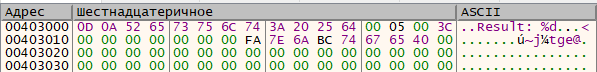
\includegraphics[width = 1 \textwidth]{picture/adress.png}
    \end{figure}


    \begin{table}[h!]
        \centering
        \caption{Шестнадцатеричный дамп памяти с выделением переменных}
        \label{tab:hexdump}
        \small
        \begin{tabular}{l cccc l}
        \toprule
        Адрес & \multicolumn{4}{c}{Шестнадцатеричное} & ASCII \\
        \cmidrule(lr){2-5}
        00403000 & 
        \cb{yellow}{0D} \cb{yellow}{0A} \cb{pink}{52} \cb{pink}{65} &
        \cb{pink}{73} \cb{pink}{75} \cb{pink}{6C} \cb{pink}{74} &
        \cb{pink}{3A} \cb{pink}{20} \cb{pink}{25} \cb{pink}{64} &
        \cb{purple!30}{00} \cb{blue!30}{05} \cb{blue!30}{00} \cb{red}{3C} &
        ..Result: \%d...< \\
        00403010 & 
        \cb{red}{00} \cb{red}{00} \cb{red}{00} \cb{green}{00} &
        \cb{green}{00} \cb{green}{00} \cb{green}{00} \cb{cyan}{FA} &
        \cb{cyan}{7E} \cb{cyan}{6A} \cb{cyan}{BC} \cb{cyan}{74} &
        \cb{cyan}{67} \cb{cyan}{65} \cb{cyan}{40} 00 &
        .......~j4tge@. \\
        00403020 & 00 00 00 00 & 00 00 00 00 & 00 00 00 00 & 00 00 00 00 & ................ \\
        00403030 & 00 00 00 00 & 00 00 00 00 & 00 00 00 00 & 00 00 00 00 & ................ \\
        \bottomrule
        \end{tabular}
    \end{table}